\subsection{Trigonometry}
\begin{align*}
\sin(v+w)&{}=\sin v\cos w+\cos v\sin w\\
\sin(v-w)&{}=\sin v\cos w-\cos v\sin w\\
\tan(v+w)&{}=\dfrac{\tan v+\tan w}{1-\tan v\tan w}\\
\sin v+\sin w&{}=2\sin\dfrac{v+w}{2}\cos\dfrac{v-w}{2}\\
\cos v+\cos w&{}=2\cos\dfrac{v+w}{2}\cos\dfrac{v-w}{2}
\end{align*}

\subsection{Triangles}
$S=\sqrt{p(p-a)(p-b)(p-c)}$, 
$S=\dfrac{abc}{4R} = pr$\\

Length of median: $m_a=\tfrac{1}{2}\sqrt{2b^2+2c^2-a^2}$\\

\subsection{Ball}
$a = \sqrt{h * (2R - h)}$, 
$V = \pi * h^2(R -\frac{h}{3})$.

\begin{center}\begin{minipage}{50mm}
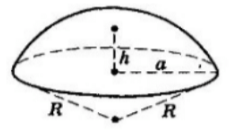
\includegraphics[width=\textwidth]{content/various/ball-segment.png}
\end{minipage}\end{center}

$V = \frac{1}{6}\pi h(3a^2+3b^2+h^2)$
$R = \sqrt{\frac{((a - b)^2 + h^2)((a + b)^2 + h^2)}{4h^2}}$

\begin{center}\begin{minipage}{50mm}
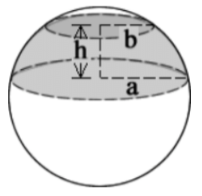
\includegraphics[width=\textwidth]{content/various/ball-layer.png}
\end{minipage}\end{center}

\subsection{Ptolemey}
$|AB| * |CD| + |BC| * |DA| \ge |AC| * |BD|$\\
Equality when ABCD on a circle.
 
